\begin{tikzpicture}
\shorthandoff{>}
%
% Concavidad de - u ln u
\begin{scope}[xscale=6.5,yscale=3.5]
\pgfmathsetmacro{\u}{.25};
\pgfmathsetmacro{\v}{1};
\pgfmathsetmacro{\l}{.7};
%
\draw[>=stealth,->] (-.1,-.5)--(1.6,-.5) node[right]{\small $t$};
\draw[>=stealth,->] (0,-.6)--(0,.5) node[above]{\small $\phi(t)$};
\draw[thick,domain=.005:1.2,samples=200] (0,0)-- plot (\x,{\x*ln(\x)});
\draw[dotted] (\u,-.55) node[below]{\small $u$} -- (\u,{\u*ln(\u)});
\draw[dotted] (\v,-.55) node[below]{\small $v$} -- (\v,{\v*ln(\v)});
%
%\draw (\u,{-\u*ln(\u)})--(\v,{-\v*ln(\v)});
\draw (.02,{(.02-\u)*(\v*ln(\v)-\u*ln(\u))/(\v-\u)+\u*ln(\u)})
-- (1.25,{(1.25-\u)*(\v*ln(\v)-\u*ln(\u))/(\v-\u)+\u*ln(\u)})
node[right,scale=.7]
{$\displaystyle \quad \frac{\phi(v)-\phi(u)}{v-u} \, (t-u) + \phi(u)$};;
%
%\draw ({.5*(\u+\v)},{.5*(\v-\u)*(\u*ln(\u)-\v*ln(\v))/(\v-\u)-\u*ln(\u)-.05})
%node[below,scale=.7]{$\displaystyle \phi(u) + (t-u) \, \frac{\phi(v)-\phi(u)}{v-u}$};
%
\draw (.02,{(1+ln(\u))*(.02-\u)+\u*ln(\u)})--
(.5,{(1+ln(\u))*(.5-\u)+\u*ln(\u)})
node[right,scale=.7]{$\quad \phi'(u) \, (t-u) + \phi(u)$};
\end{scope}
%
%
% % Concavidad / mezcla
% \begin{scope}[xshift=8.5cm]
% \draw(0,1.25) node{\includegraphics[width=3cm]{TIKZ_SZ/DosDados}};
% \draw(-.5,2.5) node{\small $p_1$};
% \draw(1,2) node{\small $p_2$};
% \draw(2.7,1) node{\small $\lambda p_1 + (1-\lambda) p_2$};
% \draw(-.25,-1) node{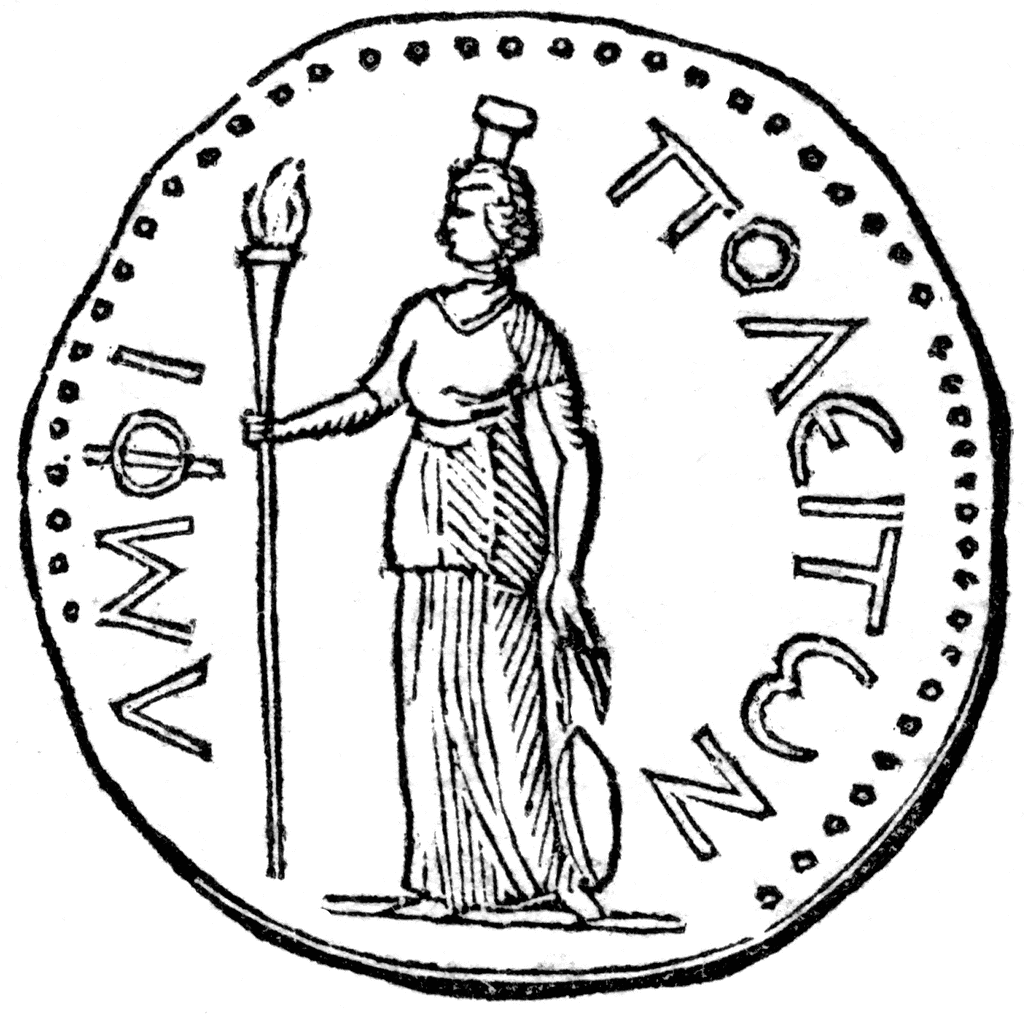
\includegraphics[width=1cm]{TIKZ_SZ/Moneda}};
% \draw[>=stealth,->,thick] (-.3,-.35)--(-.75,.45);
% \draw (-.525,0) node[left]{\small $\lambda$};
% \draw[>=stealth,->,thick] (-.2,-.35)--(.3,.45);
% \draw (.05,0) node[right]{\small $1-\lambda$};
% \end{scope}
% %
% \draw (1.25,-2.25) node{(a)};
% \draw (8.25,-2.25) node{(b)};
\end{tikzpicture}